\subsection{Dinámica}
    A partir de la expresión (\ref{eqn:DL_final}) considerando el \emph{principio de D'Alamabert-Lagrange} para sistemas con efectos de
    disipación y potencial gravitacional conservativo. Puede construirse el modelo dinámico del sistema 
    \begin{equation}
        \label{eqn:modelo_dinamico}
        \boldsymbol{\ddot{q}} =H(\boldsymbol{q})^{-1} \left \{ \boldsymbol{\boldsymbol{\tau}} - C(\boldsymbol{q}, \boldsymbol{\dot{q}}) \boldsymbol{\dot{q}}
        - D(\boldsymbol{q}, \boldsymbol{\dot{q}}) - \boldsymbol{g}(\boldsymbol{q}) \right \}
    \end{equation}
    donde el vector de torques $\boldsymbol{\tau}$ representa la entrada del sistema y $\boldsymbol{\ddot{q}}$ la salida del mismo. 
    
    Para realizar la simulación, es necesario obtener de manera simbólica en función de $(\boldsymbol{q}, \boldsymbol{\dot{q}})$ la estructura
    de cada término en (\ref{eqn:modelo_dinamico}). 

    \subsubsection{Matriz de inercia simbólica}
    Para obtener la matriz de inercia en términos de las coordenadas generalizadas, se optó por construir la función (Ver Anexo \ref{cd:inercia}) con base a la expresión
    (\ref{eqn:inertia_matrix}). De este modo, al integradar dos veces la aceleración $\boldsymbol{\ddot{q}}$ podrá utilizarse para evaluar $H(\boldsymbol{q})$
    mediante el uso de \emph{Simulink}. 

    Donde los valores de los jacobianos geométricos para cada centro de masa está dado por (\textbf{eq jacobianos geométrico}), mientras que los tensores de inercia (con valores
    en el Anexo \textbf{ANEXO Tensores de Inercia}) de cada eslabón fueron obtenidos mediante el análisis de propiedades físicas de \emph{SolidWorks}.

    \subsubsection{Vector de Coriolis simbólico}
    Una vez obtenida la matriz de inercia de manera simbólica, puede procederse con el cálculo del vector de Coriolis $C(\boldsymbol{q}, \boldsymbol{\dot{q}})$ mediante
    los símbolos de Christoffel expuestos en (\ref{eqn:christoffel}) tal como se presenta en la función de \emph{MATLAB} del Anexo \ref{cd:coriolis}. 

    \subsubsection{Vector de disipación}
    Mientras que el vector de disipación $D(\boldsymbol{q}, \boldsymbol{\dot{q}})$ está basado en la expresión (\ref{eqn:disipacion_simple}) con coeficientes de fricción
    viscosa iguales para cada articulación; suponiendo así, que la fricción dado el rozamiento entre componentes mecánicos y el motor es la misma para cada articulación. 

    Cabe destacar que $b$ es un parámetro que el usuario podrá modificar en un intérvalo de $0$ a $0.1$ $[\frac{Ns}{m}]$, con el fin de tener un análisis más amplio sobre
    el robot. Por lo que al tener un valor de $b=0$, se asume que el sistema no perderá energía dados los efectos de disipación y por ende, se estará hablando de un sistema
    conservativos. 

    \subsubsection{Vector de gravedad simbólico}
    Como último componente del modelo dinámico, $\boldsymbol{g}(\boldsymbol{q})$ fue obtenido a partir de la expresión (\ref{eqn:vector_gravedad}). Donde
    \begin{equation}
        \label{eqn:g_0}
         \boldsymbol{g}_0 = \begin{bmatrix} 0 & 0 & -9.81 \end{bmatrix}^T
    \end{equation}
    está en coordenas inerciales con unidades en $[\frac{m}{s^2}]$. Su construcción se presenta en el Anexo \ref{cd:gravedad}.

    \subsubsection{Diagrama de bloques}
    Considerando que \emph{Simulink} funciona mediante bloques, cada una de los términos requeridos por (\ref{eqn:modelo_dinamico}) pueden ser exportados mediante la
    función \emph{matlabFunctionBlock} \cite{matlabFunctionBlock}. Por lo que al implementarse, se obtiene el diagrama de bloques de la Figura \ref{fig:diagrama_bloques}.
    \begin{figure}[H]
        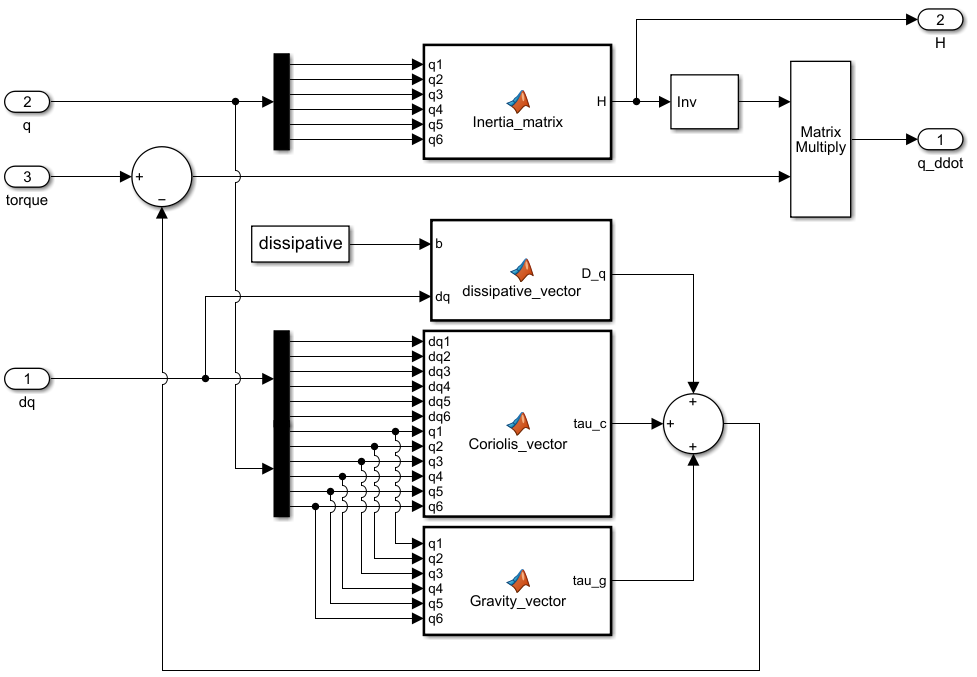
\includegraphics[scale = 0.38]{diagrama_bloques.png}
        \centering
        \caption{Diagrama de bloques del modelo dinámico}
        \label{fig:diagrama_bloques}
    \end{figure}
    Donde \emph{dissipative} representa al factor de disipación $b$ indicado por el usuario, $dq$ indica $\boldsymbol{\dot{q}}$ y \emph{torque} es equivalente a
    $\boldsymbol{\tau}$.

    Sin embargo, 
